\newpage
\partie{1}
\section{Creation Des Tables}
\subsection{Sportifs}
\lstinputlisting{Parties/Partie1/CreateTables/createSportifs.sql}

\vspace{0.25cm}

\subsection{Sports}
\lstinputlisting{Parties/Partie1/CreateTables/createSports.sql}

\vspace{0.25cm}

\subsection{Gymnases}
\lstinputlisting{Parties/Partie1/CreateTables/createGymnases.sql}

\vspace{0.25cm}

\subsection{Arbitrer}
\lstinputlisting{Parties/Partie1/CreateTables/createArbitrer.sql}

\vspace{0.25cm}

\subsection{Entrainer}
\lstinputlisting{Parties/Partie1/CreateTables/createEntrainer.sql}

\vspace{0.25cm}

\subsection{Jouer}
\lstinputlisting{Parties/Partie1/CreateTables/createJouer.sql}

\vspace{0.25cm}

\subsection{Seances}
\lstinputlisting{Parties/Partie1/CreateTables/createSeance.sql}

\newpage

\textbf{\underline{Verification Des Table Crees}}
\vspace{1cm}
\begin{center}
    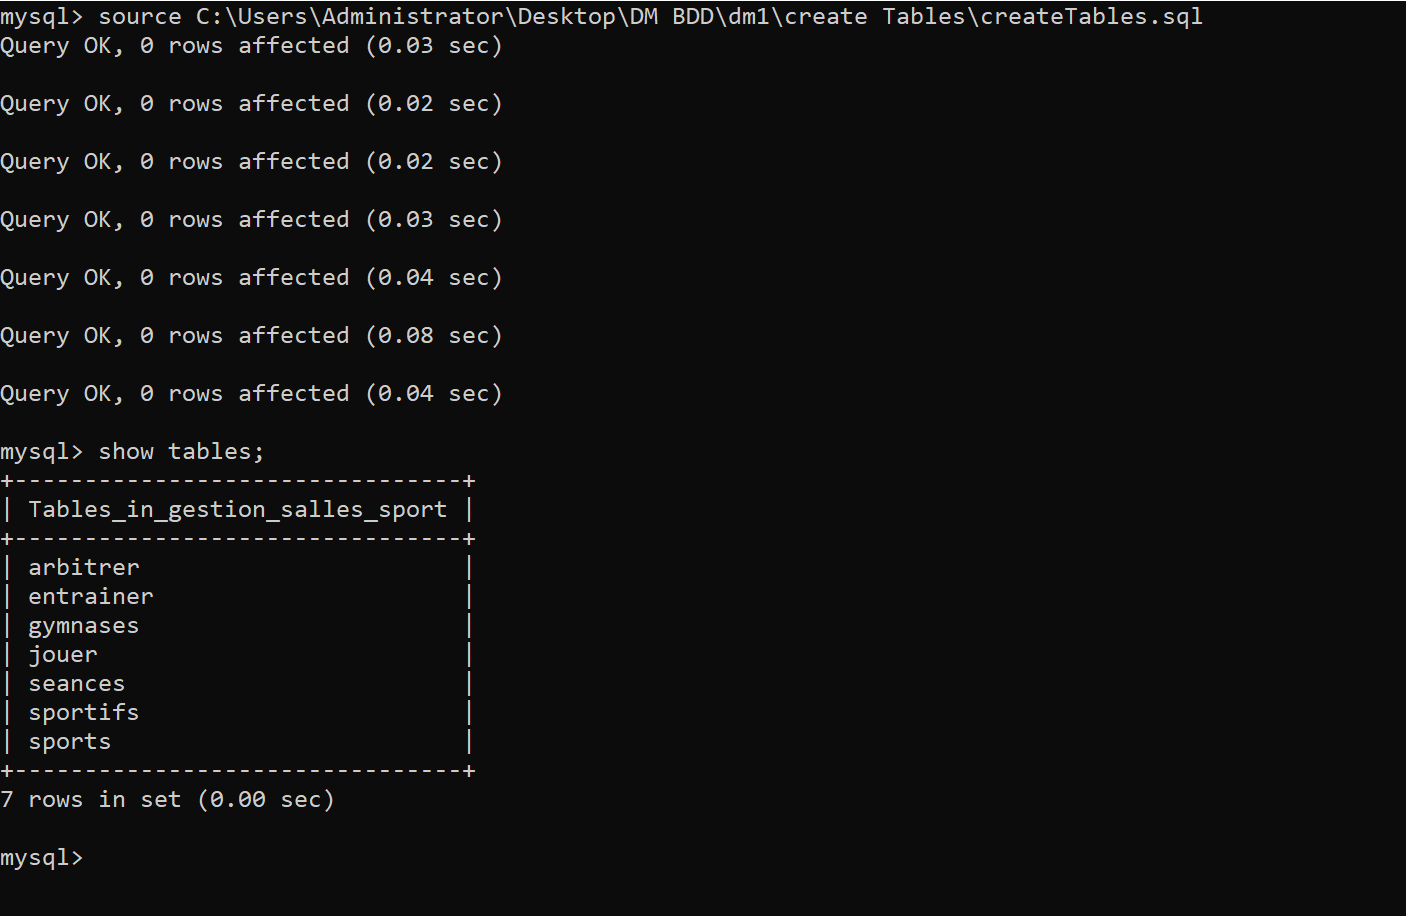
\includegraphics[height=0.6\textheight]{Parties/Partie1/CreateTables/showTables.PNG}
\end{center}

\newpage
\section{Ajouter L'attribut \texttt{DateCreation} A La Table \texttt{Gymnases}}
\lstinputlisting{Parties/Partie1/q2.sql}

\vspace{1cm}
\section{Ajouter La Contrainte \texttt{Not Null} Aux Attributs \texttt{SEXE} et \texttt{Age} De La Table \texttt{Sportifs}}
\lstinputlisting{Parties/Partie1/q3.sql}

\vspace{1cm}
\section{Modifier La Taille De L'Attribut \texttt{Prenom} De La Table \texttt{Sportifs}}
\lstinputlisting{Parties/Partie1/q4.sql}

\vspace{1cm}
\section{Suppression De L'attribut \texttt{DateCreation} A La Table \texttt{Gymnases}}
\lstinputlisting{Parties/Partie1/q5.sql}

\vspace{0.25cm}
\textbf{\underline{Output}}
\vspace{0.25cm}
\begin{center}
    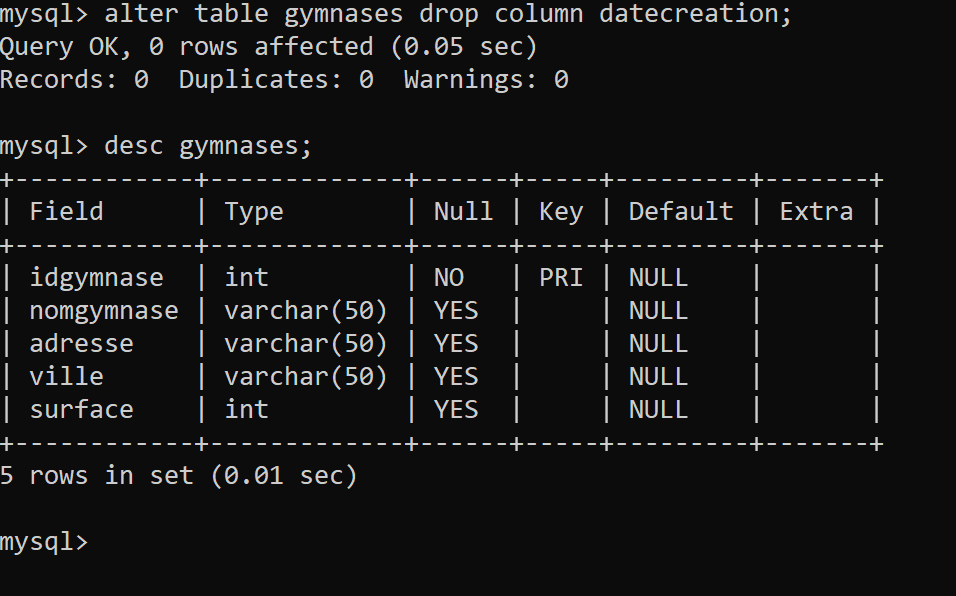
\includegraphics[height=0.36\textheight]{Parties/Partie1/drop.PNG}
\end{center}

\newpage

\section{Renommer L'attribut \texttt{ADRESSE} A La Table \texttt{Gymnases} Par \texttt{ADRESSEGYM}}
\lstinputlisting{Parties/Partie1/q6.sql}

\vspace{0.25cm}
\textbf{\underline{Output}}
\vspace{0.25cm}
\begin{center}
    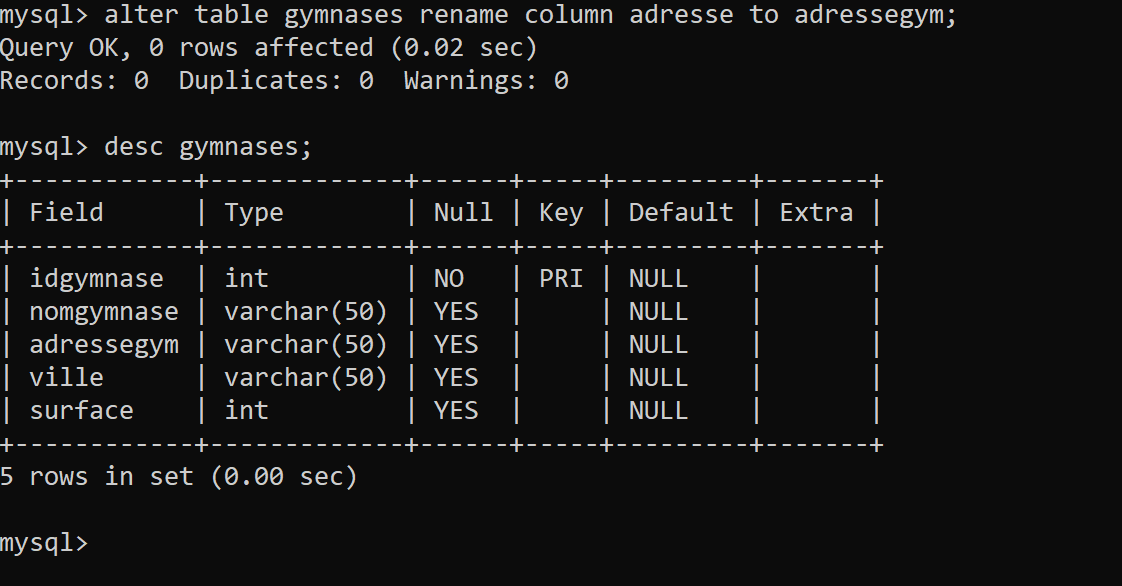
\includegraphics[height=0.36\textheight]{Parties/Partie1/rename.PNG}
\end{center}


\vspace{1cm}

\section{Ajouter La Contrainte \texttt{Check} A L'Attribut \texttt{LIBELLE} De La Table \texttt{Sports}}
\lstinputlisting{Parties/Partie1/q7.sql}



